%concepts
Task B3 was to implement a non-premptive scheduler. We will first look into at what a scheduler is and what it does.

\subsection{The scheduler}
A conservative definition of a CPU says that it executes code in a linear form, meaning that all program code needs to be written/executed sequentially. Therefore there can only be executed one program at once, using up all of the CPU's processing power, which often is in abundance. It the program is waiting for an I/O device, letting it execute would lower the overall performance of the system. This is one of the main reasons for using scheduling. Today most operating systems have the ability to run many programs simultaneously without significant loss of performance or user experience.\\
\\
This is made possible by the scheduler, whose job is to divide the processing power of the CPU to the many processes and threads that may require it. The "simple" CPU still only manages to run its assigned code sequentially, but the scheduler can assign what code to run - That's its job. Scheduling can be done using various different algorithms.

% Agreed - but we should write this in a comment
% !!!!!!Maybe write a short intro to scheduling algorithms!!!!!!!!
\subsubsection{Non-preemptive}
Threads are allowed to run until it is finished or goes into blocked state on its own. A thread may for example block when requesting an I/O operation or calling the sleep system call.
\\
This means that any other thread will have to wait indefinitely until all preceding threads have gone into blocked state or have finished. 

\subsubsection{Preemptive}
Instead of allowing threads to run indefinitely, we halt them during execution to allow another thread to run. For this to be viable, a hardware interrupt is required. When the scheduler interrupt is received by the CPU, it is handled by the scheduler interrupt code. The scheduler then saves all the relevant registers, including the program counter. This is referred to as a context switch, and allows return the thread and its state, at any time.

\subsubsection{Round robin}
Now that the scheduling concept is defined, we need to figure out which thread to run and when. There are many scheduling algorithms defined, all with different strengths and weaknesses. Our implementation is referred to as round robin and is a very simple in that is only cycles thru all threads in the ready state and assigns them CPU runtime. The round robin algorithm has no prioritizing in its basic implementation, and therefore all threads are treated equally in the queue and no thread is skipped or delayed CPU time.

\subsubsection{Priority}
For some "critical" applications it is more important that it gets more CPU time. These critical applications often need this extra attention, so that the user experience isn't negatively affected. An example of this is the mouse cursor, which needs to move seamlessly across the screen in a single flowing motion. Therefore many algorithms support thread prioritizing in some form, allowing highest priority threads ahead of all others with lower priority.

\subsubsection{Process states}
In this section we will explain a little about the different states that processes can have when being handled by the scheduler. Since our implementation of the kernel is able to handle multiple threads per process, we will be referring to thread states, as appose to single-threaded-processes. This just means that we do not look at processes, but just the states of individual threads. We will also in this section make the assumption, that a scheduler implements some kind of time-sharing for the CPU, so that each thread gets the same amount of processing time
\\
\\
When running multiple threads with the help of a scheduler, the CPU processing time is reduced, each time a thread is added to the scheduler queue. Since CPU time is precious, it is good practice to not waste resources on threads that don't require processing. Probably the simplest example is when code that needs to sleep/pause/wait before continuing its code execution. The program can in this case voluntary make a call to the operating system telling it to skip all its execution for a designated time period. This is also referred to as setting the thread state to blocked.
\\
\\
Another reason for halting execution is when some kind of data is missing, which is vital for continue execution. This could be that an application is waiting for I/O data, and a time delay is on that operation. Instead of having the application check for incoming data at timed intervals, we could have the operating system handle the I/O call, and block the thread until the data is available.
\\
\\
Threads can be in one of three states; running state, ready state or blocked state.
When a thread is in the running state, it is being executed by the CPU. It can from this state go to block or ready, depending on the circumstances. The ready state is for threads that are waiting for CPU time. It is then up to the scheduler which threads with ready state are executed by putting them in running state. Threads that already are in the blocked state and are designated to be run are returned to the ready state, and the scheduler takes over, as with all other threads in ready state.
\\
\\
\begin{figure}
\centering
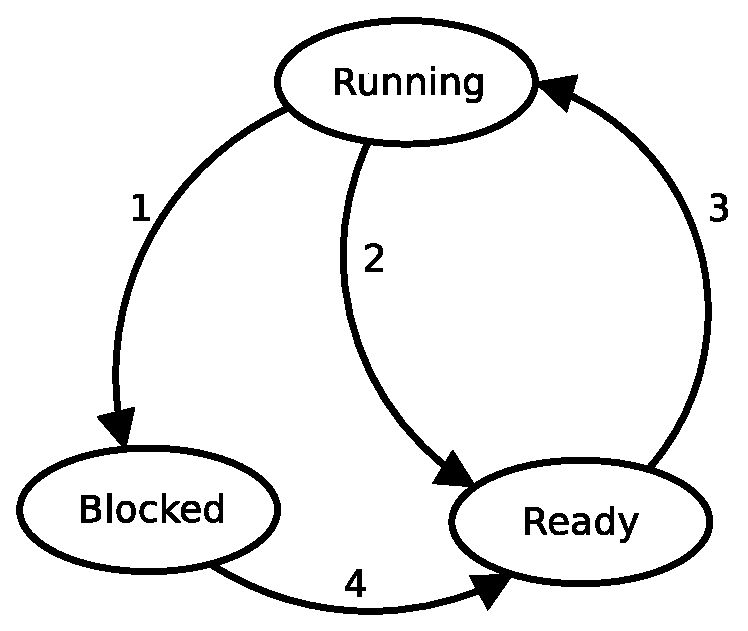
\epsfig{file=fig/Process_states.eps, height=1.5in}
\caption{Process states}
\label{fig:process_states}
\end{figure}

\subsection{Implementation}
\subsubsection*{scheduler.c}
The non-preemptive scheduler is implemented in the scheduler.c file, which is then included in the kernel.c file, in the system\_{}call\_{}handler() function. This means that scheduling occurs after each system call. We can also force a reschedule, which means that the currently running thread will not execute and will not be put into the ready\_{}queue. In other words the currently running thread will go into blocked state.
We make use of the variable schedule to indicate whether we want to force a rescheduling or not. If it's set to one, we don't add the currently running thread to the ready queue, i.e. the thread is in blocked state. Otherwise we enqueue the thread in the ready queue.

\subsubsection*{pscheduler.c}
At each interrupt the kernel decrements the tickets left for the current thread. If the ticks have decremented to 0 or below, then it is time to change to another thread. So the current thread is placed at the back of the running queue so that the next thread can be de-queued and set to run. Once the thread\_index variable has been set, the predefined timeslice ticker is reset and the whole procedure repeats itself on the next timed interrupt.



\subsection{Reflections}

\subsubsection*{What is a scheduler? What does it do and how does it work?}
A scheduler is a piece of software that shares cpu time to threads in some way. It works by keeping track of the currently running and all ready threads. If the current threads timeslot is up or it blocks, it schedules a new thread.
\subsubsection*{Assume a thread can be in three different states: running, blocked, ready. Between the states, there are various transitions. Relate the states and transitions to the code and actions in the system.}
Transition 1: The thread goes into blocked state. This is handled by the system call pause. When we call pause the thread will be inserted into the timer queue, which is a linked list of the currently paused threads, based on how many ticks it is paused for.  The head of the timer queue is the thread that has the least amount of ticks left.\\
Transition 2: The thread goes from running state to ready state. This is handled by the scheduler. The thread is enqueued into the ready queue.\\
Transition 3: The thread goes into running state. This is again handled by the scheduler. The head of the ready queue is dequeued and set to execute.\\
Transition 4: The thread goes from blocked to ready state. This is handled in the interrupt handler. It checks if there are any threads that should be woken up. If there are, it removes them from the timer queue and inserts them into the ready queue.

\subsubsection*{How does the thread queue data type work?}
The thread queue data type has a head and tail. These correspond to a thread index. It uses the next field in the thread union to construct a linked list. This linked list can then be manipulated with the functions defined in threadqueue.h.\\
\subsubsection*{How does the timer queue work?}
The timer queue is a linked list that contains all the currently paused threads. The head of the list has a list\_{}data field that specifies how many ticks are left before it should be made ready. The next thread has a list\_{}data field that contains the amount of ticks left after the previous thread has been made ready. So if we want to find out how many ticks are left before a random thread is made ready, we have to add the list\_{}data fields of all the previous thread together.\\


\subsubsection*{How does preemption influence the design of an operation system? How does it influence the scheduler?}
Preemption will influence the design of an operating system in many ways, depending on the type of system. Is the system designed for high interactivity, or maybe for batch processing? The designer will have to make some decisions regarding when and what to preempt. Should it be possible to preempt the kernel? \\
\\
The scheduler will have to change as well. It has to be able to be invoked from the interrupt handler. There also has to be some kind of bookkeeping of how long a process or thread has been executing. \\
\\
In our case the scheduler has to check if the thread has used up its timeslice. If it has, a new thread will be scheduled to run.

\subsubsection*{How would the scheduler change if the system was to support processes with real-time requirements?}
Our preemptive scheduler implementation has a very basic implementation which only uses a round-robin order when determining which thread to schedule. As is, the scheduler treats every thread with equal importance, meaning that it is not priority based, and the thread queue has the same order every cycle - threads are executed in same order every time.\\
\\
If the operating system was a real-time system, then most likely a more advanced scheduler would be implemented which would treat threads with different importance. This is usually referred to as a priority based scheduler, and can be implemented in many different ways, depending on the system requirements.\\
\\
It is difficult to go into specifics regarding a priority based system, but it simply boils down to setting individual priority for threads, and having the threads with highest priority supersede those with lower priority – Thereby ``dynamically'' changing the order of the thread queue.

\subsection{Test}
The two executables should print out different strings, where one prints “ping” and the other “pong”. One of the processes simply goes into a unconditional loop and waits a curtain amount of ticks with the sleep system call, before printing its “Pang” string. The other process goes into a unconditional loop that uses another loop to busy the CPU for 100 ticks, before it prints its “Ping” string. The  Since the kernel is running on a preemptive scheduler, the outputs from the two schedulers should alternate, depending on the loop and sleep conditions. This desired result was achieved as defined in task definition, and the test was a success.